\documentclass[10pt]{article}
\usepackage[italian]{babel}
\usepackage{array}
\usepackage{graphicx}
\usepackage[export]{adjustbox}
\usepackage{ragged2e}
\usepackage{float}
\usepackage[hidelinks]{hyperref}
\usepackage{caption}
\usepackage{listings}
\usepackage{xcolor}
\usepackage{subcaption}

\usepackage{fancyhdr}
\pagestyle{fancy}

\setlocalecaption{italian}{contents}{Indice}


% Imposta intestazioni
\fancyhead[L]{Lorenzo Maria Pennelli}        % L = left
\fancyhead[R]{Laboratorio di Algoritmi e Strutture Dati} % R = right
\begin{document}

\par\medskip
\begin{center}

\includegraphics[scale=0.1,center]{unifilogo/firenze2}
\end{center}

\begin{center}
\par\medskip
\textsc{{\large Università degli studi di Firenze}}\\
\par\medskip
\textsc{{\normalsize Dipartimento di Ingegneria Informatica}}\\
\par\medskip
\par\medskip
\hrule width 12cm height 1pt \par
\par\medskip
\par\medskip
\par\medskip
{\Huge \textbf{Statistiche d'ordine dinamiche}}\\
\par\medskip
\par\medskip
\par\medskip
\hrule width 12cm height 1pt \par
\par\medskip
\par\medskip
\par\medskip
\par\medskip
\emph{Autori:} \hfill \emph{Docente corso:}\\
\par\medskip
Pennelli Lorenzo Maria \hfill Marinai Simone\\
\par\medskip
\par\medskip
\emph{N. Matricola:} \hfill \emph{Corso principale:}\\
\par\medskip
7078749 \hfill Algoritmi e Strutture dati
\end{center}
\newpage

\tableofcontents
\listoffigures
\listoftables
\newpage

\section{Introduzione}
\label{introduzione}
\subsection{Descrizione teorica del problema}
Il progetto assegnato consiste nel confrontare le funzioni di statistiche di ordine dinamiche, \textbf{OS-Select} e \textbf{OS-Rank}, su tre strutture dati.
In particolare abbiamo trattato come strutture dati:
\begin{itemize}
\item \textbf{Lista Ordinata} (è stata implementata con i puntatori).
\item \textbf{Albero Binario di Ricerca standard} (senza attributi aggiuntivi).
\item \textbf{Albero Rosso Nero con l'attributo size}
\end{itemize}
I test sono stati realizzati in linguaggio Python. 
\newline
La relazione che segue, presenta inizialmente in modo sintetico una trattazione teorica di ciò che sarà valutato negli esperimenti, poi seguirà la documentazione del codice relativo all'implementazione delle strutture dati e dei codici di test.
Successivamente è presente l’osservazione dei risultati dei test, dove verranno valutati i risultati ottenuti con le loro aspettative teoriche.

\subsection{Specifiche della piattaforma di test}
La piattaforma di test sarà la stessa per ogni esercizio che vedremo. Partiamo dall’hardware del computer fondamentale da conoscere per questo esercizio:
\begin{itemize}
    \item \textbf{CPU}: Intel(R) Core(TM) i7-9750H CPU @ 2.60GHz
    \item \textbf{RAM}: 8GB Dual DDR4 
    \item \textbf{SSD}: 237GB
\end{itemize}
L'ambiente in cui è stato scritto e testato il codice è l'IDE \textbf{PyCharm 2023.3.4}. La stesura di questo testo è avvenuta con l'utilizzo dell'editor online \textbf{Overleaf}.
\newpage

\section{Trattazione Teorica}
\subsection{Definizioni delle funzioni Select e Rank}
Come spiegato nell'\hyperref[introduzione]{introduzione} in questo progetto valuteremo in particolare le funzioni di \textbf{OS-Select} e di \textbf{OS-Rank}. Funzioni basilari per le Statistiche d'Ordine Dinamiche.
\begin{itemize}
\item \textbf{OS-Select(S, i)}: restituisce l’i-esimo elemento più piccolo in un insieme ordinato.
\item \textbf{OS-Rank(S, x)}: restituisce la posizione dell'elemento $x$ in un insieme ordinato.    
\end{itemize}
Troviamo la loro utilità nel cercare o determinare la posizione in dataset di grandi dimensioni o con  dimensioni sempre variabili. Grazie a loro possiamo sempre sapere il minimo, il massimo e la mediana. \textit{(Nelle sezioni successive per semplicità OS-Select e OS-Rank verranno chiamati Select e Rank)}.

\subsection{Implementazione su Strutture Diverse}
Abbiamo confrontato 3 diverse implementazioni di statistiche d'ordine dinamiche per vedere come variano in base alla struttura dati. Le strutture dati prese in esame sono: \textbf{Lista ordinata}, \textbf{Albero Binario di Ricerca standard}, \textbf{Albero Rosso Nero aumentato con l'attributo Size}.
\paragraph{Lista Ordinata (lista collegata ordinata)}
Questa struttura mantiene gli elementi ordinati in maniera crescente, utilizzando i puntatori tra i nodi.

\begin{itemize}
    \item \textbf{Select(S, i)}: per accedere all’elemento in posizione $i$, è necessario scorrere sequenzialmente i primi $i$ nodi. \\
    \textbf{Complessità}: $O(i)$ e nel caso peggiore $O(n)$
    
    \item \textbf{Rank(S, x)}: per contare quanti elementi sono minori o uguali a $x$, si deve scorrere tutta la lista confrontando ciascun nodo. \\
    \textbf{Complessità}: $O(n)$
\end{itemize}

\noindent \textit{Considerazioni:} semplice da implementare, ma inefficiente per dataset di grandi dimensioni.

\vspace{0.5cm}

\paragraph{Albero Binario di Ricerca (BST)}
Struttura gerarchica in cui ogni nodo ha un figlio sinistro con valori minori e un figlio destro con valori maggiori. Tuttavia, non mantenendo informazioni aggiuntive come la dimensione del sottoalbero, le operazioni statistiche risultano complesse.

\begin{itemize}
    \item \textbf{Select(S, i)}: senza l’attributo \texttt{size}, si deve effettuare una visita \textit{in-order} fino a raggiungere il nodo in posizione $i$. \\
    \textbf{Complessità}: $O(n)$
    
    \item \textbf{Rank(S, x)}: si conta quanti nodi hanno valore minore o uguale a $x$, visitando potenzialmente l’intero albero. \\
    \textbf{Complessità}: $O(n)$
\end{itemize}

\noindent \textit{Considerazioni:} se l’albero è sbilanciato, può degenerare in una lista, peggiorando drasticamente le prestazioni.

\vspace{0.5cm}

\paragraph{Albero Rosso-Nero con attributo \texttt{size}}
Struttura bilanciata che garantisce altezza logaritmica e include un attributo \texttt{size} in ogni nodo, rappresentante la dimensione del sottoalbero radicato in quel nodo.

\begin{itemize}
    \item \textbf{Select(S, i)}: si utilizza l’attributo \texttt{size} per decidere se cercare nel sottoalbero sinistro, nel destro, o se il nodo corrente è quello cercato. \\
    \textbf{Complessità}: $O(\log n)$
    
    \item \textbf{Rank(S, x)}: seguendo il cammino di ricerca verso $x$, si sommano le dimensioni dei sottoalberi sinistri visitati e si ottiene così il rango. \\
    \textbf{Complessità}: $O(\log n)$
\end{itemize}

\noindent \textit{Considerazioni:} struttura molto efficiente, ideale per operazioni dinamiche su insiemi ordinati, grazie al bilanciamento e all’uso di attributi ausiliari.

\vspace{0.5cm}

\begin{table}[H]
\centering
\begin{tabular}{|l|c|c|}
\hline
\textbf{Struttura Dati} & \textbf{Select} & \textbf{Rank} \\
\hline
Lista Ordinata & $O(i)$ & $O(n)$ \\
Albero Binario di Ricerca & $O(n)$ & $O(n)$ \\
Albero Rosso-Nero con \texttt{size} & $O(\log n)$ & $O(\log n)$ \\
\hline
\end{tabular}
\caption{Complessità delle operazioni \texttt{Select} e \texttt{Rank} con diverse strutture dati}
\label{tab:complessita}
\end{table}
\subsection{Note sull'Albero Rosso-Nero con \texttt{size}}

L'Albero Rosso-Nero con l'attributo \texttt{size} è un classico esempio di struttura dati aumentata. L’aggiunta dell’attributo \texttt{size}, che rappresenta la dimensione del sottoalbero radicato in ciascun nodo, consente di eseguire efficientemente operazioni come \texttt{Select} e \texttt{Rank} in tempo logaritmico.

\noindent Tale modifica non altera la complessità delle operazioni fondamentali dell’albero (inserimento, cancellazione, ricerca), che rimangono anch’esse in $O(\log n)$. Questo rende l’albero rosso-nero aumentato particolarmente adatto al contesto dell’elaborazione di statistiche d’ordine, senza dover ideare strutture dati completamente nuove.

\paragraph{Limitazioni}

L’aggiunta dell’attributo \texttt{size} comporta un modesto aumento dello spazio occupato da ciascun nodo e introduce una leggera complessità nella gestione delle operazioni dinamiche. In particolare, durante l’inserimento e la cancellazione, è necessario aggiornare correttamente l’attributo \texttt{size} lungo il cammino di risalita, nonché durante eventuali rotazioni strutturali.

\noindent Tuttavia, questi aggiornamenti possono essere effettuati localmente in tempo costante per ogni nodo coinvolto, mantenendo la complessità complessiva delle operazioni pari a $O(\log n)$.


\section{Documentazione Codice}
\subsection{Struttura del progetto}

Il progetto è organizzato secondo una struttura ad albero, che suddivide logicamente i file in base alla loro funzione. Di seguito si riporta l’alberatura dei file e delle directory principali:
\begin{lstlisting}[basicstyle=\ttfamily\small, frame=none]
.
+-- input
+-- output/
|   +-- plots/
|   |    +-- LinkedList/
|   |    |   +-- random/
|   |    |   |   +-- select.png
|   |    |   |   +-- rank.png
|   |    |   +-- randomDuplicate
|   |    |   +-- sorted
|   |    |   +-- reverse
|   |    +-- BinarySearchTree
|   |    +-- confronto
|   |    +-- RedBlackTree
|   |    +-- RBTLarge
|   |    +-- table
|   +--benchmark_results.csv 
+-- StruttureDati/
|   +-- Node/
|   |   +-- NodeList.py
|   |   +-- TreeNode.py
|   |   +-- NodeRedBlack.py
|   +-- ABR.py
|   +-- OrderedList.py
|   +-- ARN.py  
+-- testFunctions/
|   +-- ARNValutation.py
|   +-- CreateInput.py
|   +-- BenchmarkSelectRank.py
|   +-- CreateTables.py 
|   +-- PlotResults.py
+-- main.py
\end{lstlisting}
\subsubsection{Directory input e output}
\begin{itemize}
    \item \textbf{Input}: Contiene i file di input utilizzati per i test sperimentali. Questi file vengono generati automaticamente da script presenti nella directory \textbf{testFunctions/CreateInput.py} che popola questa cartella di file \textbf{.joblib} che salvano le strutture dati e informazioni utili al rank. Così evitiamo di creare e ripopolare ogni volta le strutture dati.
    \item \textbf{Output}: Raccoglie tutti i risultati prodotti durante l’esecuzione degli esperimenti. Al suo interno si trova la cartella \textbf{plots/}, che contiene i grafici generati per ciascuna struttura dati e scenario di test. Inoltre, sono presenti i file csv dei tempi dei benchmark.
\end{itemize}
\subsection{Strutture Dati}
Per svolgere i nostri esperimenti ho, prima di tutto, scritto il codice delle strutture dati a cui faremo riferimento.
Le classi sono \textbf{BinarySearchTree} presente nel file \textbf{ABR.py}, \textbf{TreeRedBlack} presente nel file \textbf{ARN.py}, \textbf{OrderedLinkedList} presente nel file \textbf{ListaOrdinata.py} e poi gli eventuali nodi usati, presenti negli omonimi file, \textbf{NodeList}, \textbf{NodeRedBlack}, \textbf{TreeNode}. La classe \textbf{BinarySearchTree} rappresenta la struttura dati dell'albero di binario di ricerca e "usa" la classe \textbf{TreeNode}. La classe \textbf{TreeRedBlack} raffigura un albero rosso nero e possiede la classe \textbf{NodeRedBlack}. L'ultima struttura rimasta è la \textbf{OrderedLinkedList} che rappresenta la lista ordinata, questa lista è stata implementata senza l'uso di nessuna libreria python, ma usando \textbf{NodeList} che ci permette di creare su python una lista collegata con i puntatori grazie ai suoi attributi \textbf{left} e \textbf{right} che collegano il nodo ad altri elementi della lista. Come si può notare dal \hyperref[strDatiDiagram]{ Class Diagram} sottostante la classe \textbf{TreeNode} estende la classe \textbf{NodeList}. Stessa cosa accade tra \textbf{NodeRedBlack} e \textbf{TreeNode}. Come si potrebbe , invece, pensare, la classe \textbf{TreeRedBlack}, nonostante l'albero rosso nero possa essere visto come una versione più bilanciata di un albero binario di ricerca, non estende la classe \textbf{BinarySearchTree}. Questa scelta è dovuta al fatto che il focus dell'esperimento sia il valutare i tempi dei \textbf{Select} e dei \textbf{Rank} e quindi ho realizzato solo i metodi necessari che si sono rilevati molto diversi tra le strutture dati. 
\begin{figure}[H]
    \centering
    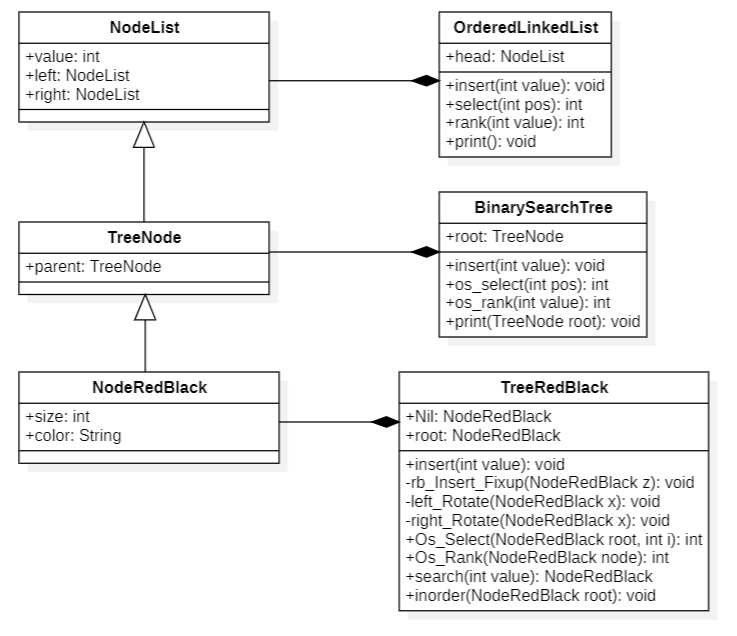
\includegraphics[width=1\linewidth]{resources/StrDiagramm.png}
    \caption{Diagramma di classe per le strutture dati}
    \label{strDatiDiagram}
\end{figure}
\subsection{Funzioni di test}
Per valutare in modo efficace le prestazioni delle varie strutture dati implementate, è stata predisposta una suite di script di test contenuti nella directory \textbf{testFunctions/}. Ognuno di questi script ha un compito specifico nel processo di generazione dei dati, esecuzione dei benchmark e produzione dei risultati grafici.
\begin{itemize}
    \item \textbf{CreateInput.py}: genera automaticamente diversi dataset da utilizzare per i test, salvandoli in formato \texttt{.joblib} all'interno della directory \textbf{input/}. I dataset variano per tipo di ordinamento (random, ordinato, inverso, con duplicati) e dimensione, al fine di valutare il comportamento delle strutture in vari scenari.
    \item \textbf{BenchmarkSelectRank.py}: è il cuore della fase sperimentale. Questo script esegue il confronto sistematico delle strutture dati, prendendo i file dalla cartella \textbf{input/} e applicando operazioni di \texttt{Select} e \texttt{Rank} sui dataset generati. I tempi vengono registrati per ciascuna operazione, per ogni struttura dati e per ogni tipo di input in file csv.
    \item \textbf{PlotResults.py}: prende in input i file \texttt{.csv} generati e crea i grafici presenti nella cartella \textbf{output/plots/}. I grafici rappresentano l'andamento dei tempi in funzione della dimensione del dataset, distinguendo tra diversi tipi di ordinamento e struttura dati.
    \item \textbf{CreateTables.py}: genera delle tabelle riassuntive in formato \texttt{.png} che mostrano le statistiche ottenute dalle esecuzioni, organizzandole in modo che possano essere successivamente usate per un'eventuale analisi. Salvano in tabella raggruppando per operazione e tipo di ordinamento di dato i tempi confrontati di ogni struttura dati con la loro dimensione (\textit{essendo che vengono effettuati test su tante dimensioni diverse, 30, tali tabelle non verranno usate nella loro interezza , ma verranno prese in versioni più ridotte. Tuttavia se si è interessati alle tabelle in formato originale si possono ritrovare in \textbf{output/plots/tables}})
    \item \textbf{ARNValutation.py}: contiene il codice che permette di eseguire i test specifici sull’albero Rosso-Nero. Vengono calcolati i tempi delle operazioni di \textbf{Select} e \textbf{Rank} con dataset molto più grandi, tali risultati vengono salvati in un file csv e poi vengono trasformati in un grafico. Ho dovuto creare un ulteriore file apposito perché i dataset studiati nel \textbf{BenchmarkSelectRank.py} erano troppo piccoli e quindi risolti in troppo poco tempo (solo per l'albero rosso nero) avendo così dei risultati molto soggetti al rumore generato dal computer. Inoltre, ho applicato questa separazione solo per l'albero rosso nero perché con valori troppo grandi le altre strutture dati ritardavano troppo gli esperimenti e causavano spesso crash del computer o timeout.
\end{itemize}
L’esecuzione di tutti gli script è orchestrata dal file \textbf{main.py}, che funge da punto di ingresso e permette di automatizzare l’intero processo: dalla generazione dei dati all’analisi visiva dei risultati.
\newpage
\subsection{Analisi delle scelte implementative}
Nella progettazione delle classi e nella definizione delle loro relazioni gerarchiche, si è cercato di aderire il più possibile allo pseudocodice proposto nel testo "Introduzione agli Algoritmi e alle Strutture Dati Mc Graw Hill", al fine di mantenere coerenza con le specifiche teoriche e facilitare la corrispondenza tra teoria e implementazione. Infatti, nella classe \textbf{TreeRedBlack} è stato aggiunto un attributo Nil che rappresenta una sentinella (T.Nil), il cui unico scopo è quello di indicare la fine dell'albero e il padre della radice, senza generare possibili errori dovuti a gestioni sbagliate di None.
\newline
\noindent \`E stata implementata come un \textbf{NodeRedBlack} che viene instanziato alla creazione di un albero rosso nero e ha i seguenti valori dei suoi attributi:
\begin{itemize}
    \item value= None
    \item color= 'Black'
    \item size= 0 \textit{(così non influenza il calcolo del size)}
    \item parent, left, right = Nill
\end{itemize}
\subsection{Descrizione dei metodi implementati}
In questa parte descrivero le funzionalità di ogni metodo delle classi di cui finora abbiamo parlato. 
\begin{itemize}
    \item \textbf{OrderedLinkedList}:
    \begin{itemize}
         \item \textbf{insert(value)}: Inserisce un nuovo nodo nella lista mantenendo l'ordine crescente. Se la lista è vuota, il nodo diventa la testa. Se il valore è minore della testa, viene inserito all'inizio. Altrimenti, viene inserito nella posizione corretta scorrendo la lista.
        
        \item \textbf{select(position)}: Restituisce il valore del nodo che si trova nella posizione indicata (indice zero-based). Scorre la lista dalla testa fino a raggiungere la posizione desiderata.

        \item \textbf{rank(value)}: Restituisce l'indice (rank) del primo nodo che ha il valore richiesto. Se il valore non è presente, restituisce \texttt{None}. È utile per capire la posizione di un elemento nella lista.

        \item \textbf{print()}: Stampa su console tutti i valori presenti nella lista, in ordine, a partire dalla testa.
    \end{itemize}
    \item \textbf{BinarySearchTree}:
    \begin{itemize}
       \item \textbf{insert(value)}: Inserisce un nodo nella posizione corretta dell’albero binario di ricerca seguendo le regole standard (valori minori a sinistra, maggiori o uguali a destra). Aggiorna i puntatori del nodo padre.
        
        \item \textbf{os\_select(position)}: Implementa la selezione dell’elemento in posizione \texttt{position} (1-based) utilizzando una visita \texttt{in-order} iterativa. Restituisce il valore del nodo che si trova in quella posizione nell’ordine crescente. Ho adottato di utilizzare la versione iterativa rispetto alla ricorsiva perché il compilatore forniva questo errore: "\texttt{\textcolor{red}{RecursionError: maximum recursion depth exceeded while 
        \newline
        getting the str of an object}}
"

        \item \textbf{os\_rank(value)}: Calcola il rango (posizione in ordine crescente) del nodo contenente il valore specificato. Scorre l’albero con una visita \texttt{in-order} fino a trovare il nodo con quel valore e restituisce la sua posizione. L'implementazione della visita \texttt{in-order} è stato implementato a livello iterativo sempre per il motivo specificato precedentemente.

        \item \textbf{print(root)}: Stampa i valori dei nodi dell’albero in ordine crescente, eseguendo una visita ricorsiva in-order a partire dalla radice.
    \end{itemize}
    \item \textbf{TreeRedBlack}:
        \begin{itemize}
        \item \textbf{insert(value)}: Inserisce un nuovo nodo rosso con valore \texttt{value} mantenendo aggiornati i campi \texttt{size} lungo il cammino di inserimento.
        \item \textbf{rb\_Insert\_Fixup(z)}: Ripristina le proprietà dell'albero rosso-nero dopo un'inserzione, gestendo i tre casi classici tramite rotazioni e ricolorazioni.
        \item \textbf{left\_Rotate(x)}: Esegue una rotazione a sinistra intorno al nodo \texttt{x}, mantenendo aggiornato il campo \texttt{size}.
        \item \textbf{right\_Rotate(y)}: Esegue una rotazione a destra intorno al nodo \texttt{y}, mantenendo aggiornato il campo \texttt{size}.
        \item \textbf{Os\_Select(node, i)}: Restituisce il valore del nodo con rango \texttt{i} a partire dal sottoalbero radicato in \texttt{node}, sfruttando il campo \texttt{size}. \`E stata adottata la versione classica presente nei normali libri di testo di Algoritmi e Strutture Dati.
        \begin{figure}[H]
            \centering
            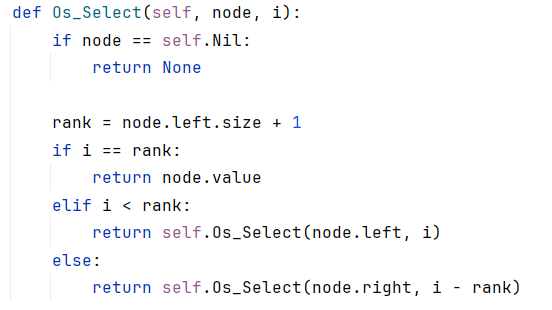
\includegraphics[width=0.65\linewidth]{resources/pseudoSelect.png}
            \caption{Funzione Select dell'Albero Rosso Nero}
            \label{select}
        \end{figure}
        \item \textbf{Os\_Rank(node)}: Calcola il rango del nodo \texttt{node} (cioè il numero di elementi minori di esso nell’albero) risalendo fino alla radice.  \`E stata adottata anche qui la versione classica presente nei normali libri di testo di Algoritmi e Strutture Dati.
        \begin{figure}[H]
            \centering
            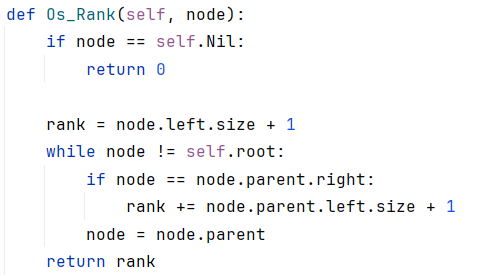
\includegraphics[width=0.65\linewidth]{resources/pseudoRank.png}
            \caption{Funzione Rank dell'Albero Rosso Nero}
            \label{rank}
        \end{figure}
        \item \textbf{inorder(node)}: Stampa in ordine crescente i valori dei nodi nel sottoalbero radicato in \texttt{node}, insieme al rispettivo \texttt{size}.
        \item \textbf{search(value)}: Restituisce il nodo con valore \texttt{value} se presente, altrimenti \texttt{None}.
    \end{itemize}
    \item \textbf{CreateInput}:
    \begin{itemize}
        \item \textbf{creation\_data\_structure()}:\\ ha il compito di generare dataset di input secondo quattro configurazioni: \texttt{random}, \texttt{sorted}, \texttt{reverse} e \texttt{randomDuplicate}. Per ciascuna di queste configurazioni, i dati vengono generati per diverse dimensioni predefinite, da 10 fino a 1400 elementi (limite massimo che la libreria joblib può gestire per salvare le strutture dati senza eccedere il proprio limite personale di ricorsione). Ogni insieme di dati viene utilizzato per popolare le tre diverse strutture dati. Dopo l'inserimento, viene eseguita l'operazione \texttt{select} su ciascuna struttura per ricavare un valore centrale (la posizione mediana, calcolata come \texttt{size // 2}). Successivamente, il valore centrale selezionato e le tre strutture dati vengono salvati su file in formato \texttt{.joblib}.
    \end{itemize}
    \item \textbf{BenchmarkSelectRank}:
    \begin{itemize}
        \item \textbf{benchmark\_from\_saved\_structures(folder, output\_csv, num\_trials)}:\\
        La funzione esegue un benchmark delle operazioni \texttt{select} e \texttt{rank} su tre strutture dati: \textbf{OrderedLinkedList}, \textbf{BinarySearchTree} e \textbf{RedBlackTree}, utilizzando i dati precedentemente salvati su file. Vengono caricati i file serializzati in formato \texttt{joblib} da una cartella specificata (default: \texttt{"input"}) e si misura il tempo medio (in millisecondi) impiegato per eseguire le due operazioni principali su ciascuna struttura. La misurazione è ripetuta per un numero di prove specificato da \texttt{num\_trials} (default: 5), per ridurre la variabilità. I risultati, contenenti tipo di dataset, dimensione, e tempi medi delle operazioni, vengono salvati in un file CSV (default: \texttt{"output/benchmark\_results.csv"}) e restituiti anche come \texttt{DataFrame} Pandas per un'eventuale analisi successiva. Sono gestiti eventuali errori durante il caricamento dei file o l'esecuzione delle operazioni.
        \begin{figure}[H]
            \centering
            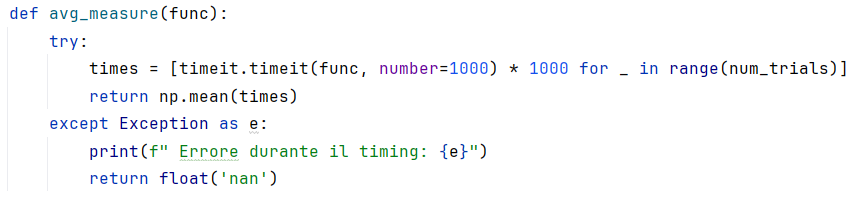
\includegraphics[width=0.85\linewidth]{resources/funzioneTempo.png}
            \caption{Funzione che misura i tempi di esecuzione}
            \label{funzione tempo}
        \end{figure}
    \end{itemize}
    \item \textbf{PlotResults}:
    \begin{itemize}
        \item \textbf{plot\_benchmarks(csv\_path)}\\
        Questa funzione si occupa di generare e salvare dei grafici a partire dai risultati di benchmark contenuti in un file CSV (default: \texttt{"output/benchmark\_results.csv"}). I dati vengono caricati in un \texttt{DataFrame} Pandas, e vengono create due tipologie principali di grafici: un confronto diretto tra tutte le strutture dati per ciascun tipo di dataset e operazione, e una visualizzazione dettagliata delle performance di ogni singola struttura per ciascun tipo di dataset.
    \end{itemize}
    \item \textbf{CreateTables}:
    \begin{itemize}
    \item\textbf{generate\_operation\_tables\_from\_csv(csv\_path, output\_folder)}\\
    Questa funzione prende in input il percorso a un file CSV contenente i risultati dei benchmark e genera tabelle comparative in formato immagine (\texttt{.png}) per ogni combinazione di operazione (\texttt{Select}, \texttt{Rank}) e tipo di dataset (\texttt{random}, \texttt{sorted}, \texttt{reverse}, \texttt{randomDuplicate}). Ogni tabella viene formattata per mostrare i tempi medi in millisecondi con precisione a 4 cifre significative e infine salvata come immagine nella cartella di output predefinita \newline
    (\texttt{output/plots/table/<operation>/<datatype>.png})
    \end{itemize}
    \item \textbf{ARNValutation}
    \begin{itemize}
        \item \textbf{benchmark\_rbt\_select\_rank(
        \newline
        trials=1000, output\_dir="output/plots/RBTLarge")}\\
        Questa funzione esegue un benchmark dettagliato delle operazioni \texttt{Select} e \texttt{Rank} su alberi Red-Black (ARN) per varie dimensioni di dati, da 100 fino a 1 milione di nodi.
        Per ogni dimensione della lista predefinita \texttt{sizes}, viene generato un dataset di numeri interi unici in ordine casuale. Successivamente, viene creato un albero Red-Black vuoto e tutti i valori del dataset vengono inseriti nell’albero. Viene quindi selezionato un valore centrale, calcolato come \texttt{i\_select = size // 2}, che viene utilizzato sia per la funzione \texttt{Select} (che esegue la ricerca per rango) sia per la funzione \texttt{Rank} (che calcola il rango di un nodo). Le funzioni \texttt{Os\_Select} e \texttt{Os\_Rank} vengono eseguite ripetutamente per un numero di volte definito da \texttt{trials}, in modo da misurarne il tempo medio di esecuzione espresso in millisecondi. I risultati dei tempi medi per ogni dimensione sono poi salvati in un DataFrame Pandas e esportati in un file CSV. Infine, la funzione genera e salva due grafici a linea, uno relativo ai tempi della funzione \texttt{Select} e l’altro ai tempi della funzione \texttt{Rank}.
    \end{itemize}
\end{itemize}
\section{Descrizione degli esperimenti condotti e analisi dei risultati sperimentali}
\subsection{Dati utilizzati}
L'esperimento che ho svolto si divide prima di tutto nel tipo di dati generati da inserire nelle strutture dati.
L'esperimento sarà diviso in 4 parti:
\begin{itemize}
    \item dati \textbf{randomici} senza duplicati.
    \item dati \textbf{ordinati} senza duplicati.
    \item dati \textbf{ordinati al contrario} senza duplicati.
    \item dati \textbf{randomici con duplicati}
\end{itemize}
Con questa divisione voglio vedere se i tempi del \textbf{Select} e \textbf{Rank} vengano influenzati dalla disposizione dei dati e se ci sono eventuali cambiamenti se siamo nel caso migliore o nel caso peggiore della struttura dati (\textit{in particolare la lista ordinata e l'albero binario di ricerca}).\newline Il range delle dimensioni delle strutture dati vanno da 10 elementi fino a 1400 osservare al meglio l'andamento con l'aumentare della dimensione.
\begin{figure}[H]
    \centering
    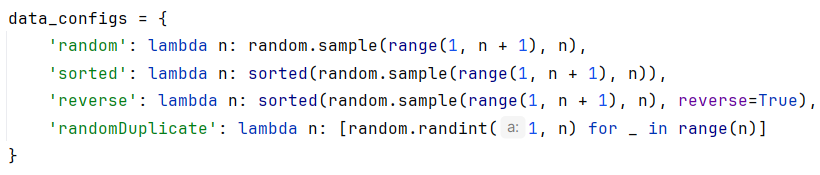
\includegraphics[width=1\linewidth]{resources/generatore dati.png}
    \caption{Frammento di codice che mostra la generazione dei dati nelle 4 casistiche in base alla dimensione}
    \label{Generator}
\end{figure}
\subsection{Risultati sperimentali}
\label{risultati sperimentali}
\subsubsection{Dati randomici senza duplicati}
Questo caso rappresenta il caso "\textbf{medio}" di tutte e tre le strutture dati. Mostriamo qui di seguito il grafico con tutte le dimensioni
\begin{figure}[H]
    \centering
    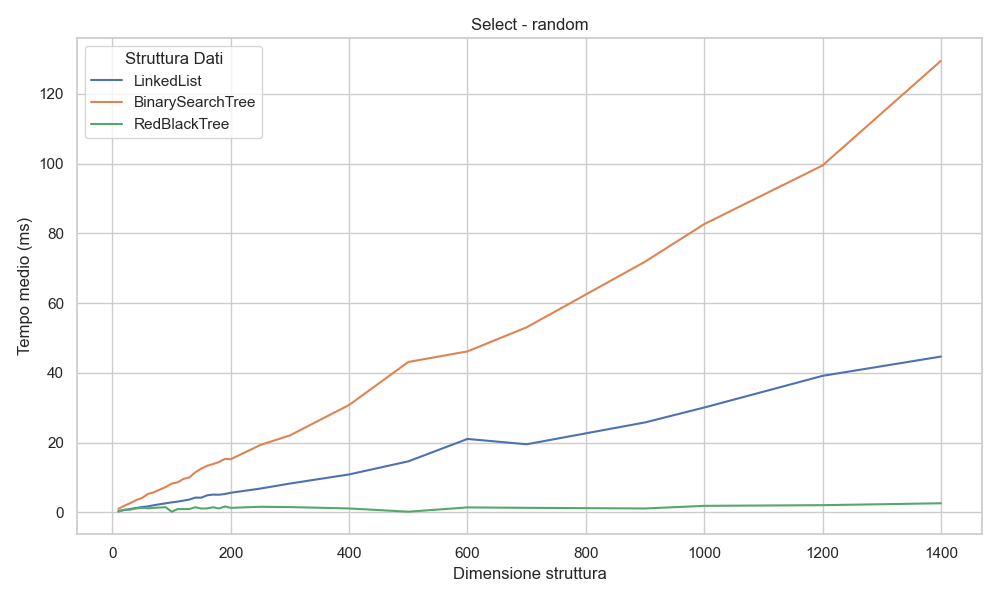
\includegraphics[width=0.8\linewidth]{plots/confronto/random_select.png}
    \caption{Grafico del Select con dati random}
    \label{confronto-select-random}
\end{figure}
\begin{table}[H]
\centering
\begin{tabular}{|c|c|c|c|}
\hline
\textbf{Size} & \textbf{Albero Binario} & \textbf{Lista Ordinata} & \textbf{Albero Rosso Nero} \\
\hline
10     & 1.054 & 0.4283 & 0.23 \\
30     & 2.681 & 1.015  & 0.8211 \\
180    & 14.47 & 5.089  & 1.144 \\
1400   & 129.5 & 44.7   & 2.643 \\
\hline
\end{tabular}
\caption{Tempi medi di esecuzione (ms) delle operazioni \texttt{Select} con dati di input random}
\label{tab:confronto_select_random}
\end{table}
\begin{figure}[H]
    \centering
    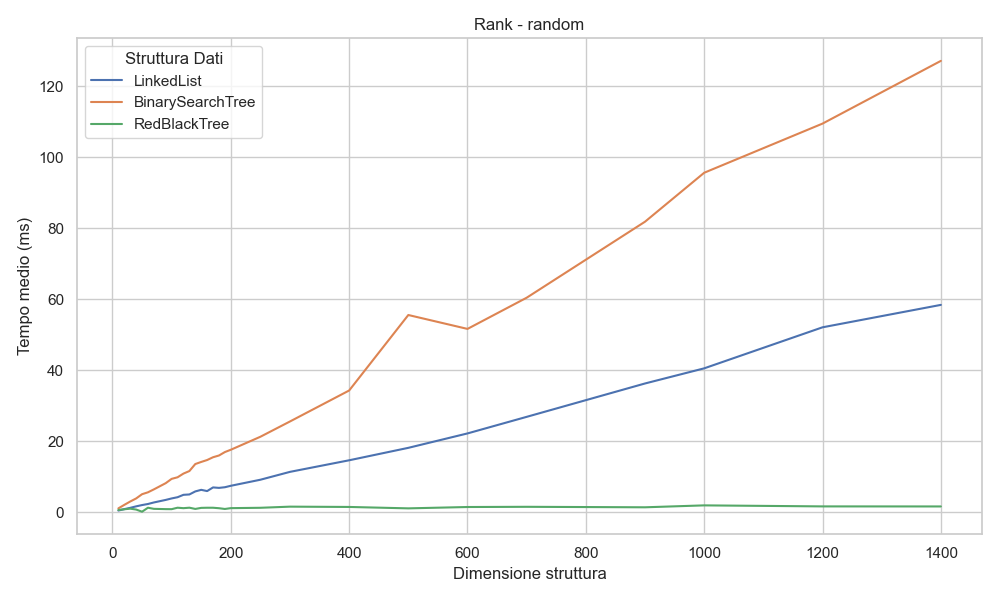
\includegraphics[width=0.8\linewidth]{plots/confronto/random_rank.png}
    \caption{Grafico del Rank con dati random}
    \label{fig:confronto-rank-random}
\end{figure}
\begin{table}[H]
\centering
\begin{tabular}{|c|c|c|c|}
\hline
\textbf{Size} & \textbf{Albero Binario} & \textbf{Lista Ordinata} & \textbf{Albero Rosso Nero} \\
\hline
10     & 1.15 & 0.535 & 0.6903 \\
30     & 3.075 & 1.295  & 1.065 \\
180    & 16.03 & 6.914  & 1.193 \\
1400   & 127.1 & 58.1   & 1.688 \\
\hline
\end{tabular}
\caption{Tempi medi di esecuzione (ms) delle operazioni \texttt{Rank} con dati di input random}
\label{tab:confronto_rank_random}
\end{table}
\begin{figure}[H]
    \centering
    \begin{subfigure}{0.49\textwidth}
        \centering
        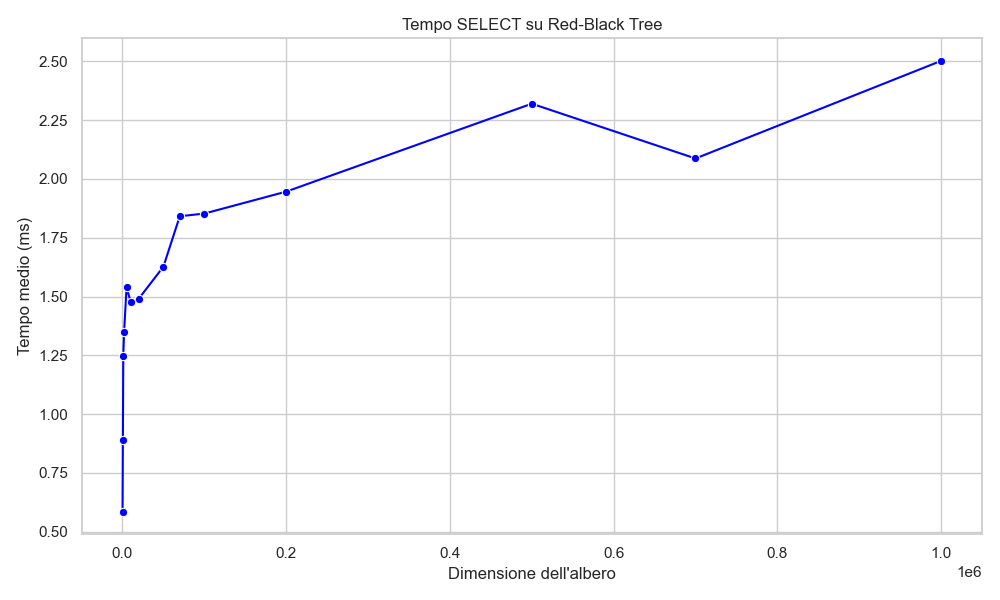
\includegraphics[width=\linewidth]{plots/RBTLarge/select.png}
        \caption{Grafico del Select dell'Albero Rosso Nero}
        \label{select-rn}
    \end{subfigure}
    \hfill
    \begin{subfigure}{0.49\textwidth}
        \centering
        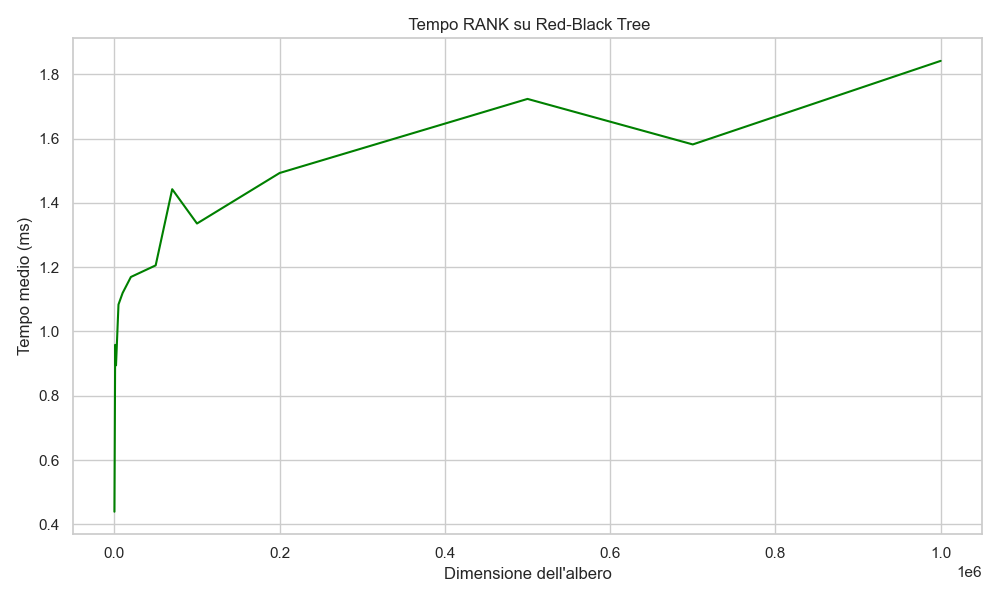
\includegraphics[width=\linewidth]{plots/RBTLarge/rank.png}
        \caption{Grafico del Rank dell'Albero Rosso Nero}
        \label{rank-rn}
    \end{subfigure}
    \caption{Tempi medi delle operazioni \textbf{Select} e \textbf{Rank} su Red-Black Tree}
    \label{fig:AlberoRNDettagliato}
\end{figure}
\noindent Notiamo dalle figure \hyperref[confronto-select-random]{6} e \hyperref[fig:confronto-rank-random]{7} che l'\textbf{albero binario di ricerca} e la \textbf{lista ordinata} hanno tempi maggiori rispetto all'\textbf{albero rosso nero}. Inoltre, queste due strutture dati, già con pochi elementi, mostrano un andamento lineare $O(n)$. La \textbf{lista ordinata} risulta leggermente più efficiente rispetto all'\textbf{albero binario di ricerca} nella funzione \texttt{Select}, soprattutto in presenza di strutture di piccole e medie dimensioni. Questo comportamento è dovuto principalmente al fatto che l'inserimento e la ricerca sequenziale in una lista collegata hanno un andamento prevedibile e lineare, mentre l'implementazione dell'albero binario di ricerca, non essendo bilanciato, può degradare in una struttura sbilanciata, con prestazioni significativamente peggiori.\newline 
L'\textbf{albero rosso nero} è talmente più efficiente che è stato valutato anche singolarmente con altri valori, anche per evitare eventuali rumori del computer, (\hyperref[select-rn]{figura 8.a} e \hyperref[rank-rn]{figura 8.b}) mostrando un andamento simil $O(logn)$. Inoltre, il diverso ordine dei dati di input non lo influenza, grazie al suo riordinamento interno (\textbf{rb\_Insert\_Fixup}) e quindi per ogni casistica di input si farà sempre esempio ai seguenti grafi.
\textit{(per maggiori informazioni \hyperref[approfondimenti]{sezione 4.3})}.

\subsubsection{dati ordinati senza duplicati}
Abbiamo preso in considerazione questo caso perché rappresenta il caso \textbf{peggiore} per l'albero binario di ricerca, dato che comporta uno sbilanciamento di quest'ultimo in una lista ordinata, e della lista ordinata. Mostriamo qui di seguito il grafico:
\begin{figure}[H]
    \centering
    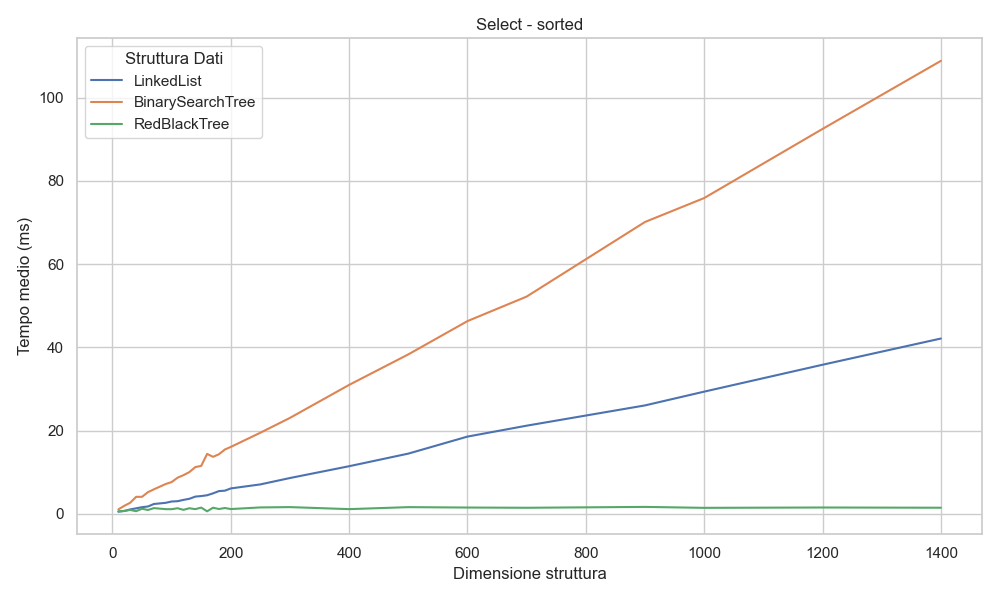
\includegraphics[width=0.8\linewidth]{plots/confronto/sorted_select.png}
    \caption{Grafico del Select con dati ordinati}
    \label{confronto-select-sorted}
\end{figure}
\begin{table}[H]
\centering
\begin{tabular}{|c|c|c|c|}
\hline
\textbf{Size} & \textbf{Albero Binario} & \textbf{Lista Ordinata} & \textbf{Albero Rosso Nero} \\
\hline
10     & 1.095 & 0.5392 & 0.6353 \\
30     & 2.692 & 1.093  & 0.962 \\
180    & 14.34 & 5.49  & 1.186 \\
1400   & 108.8 & 42.12  & 1.494 \\
\hline
\end{tabular}
\caption{Tempi medi di esecuzione (ms) delle operazioni \texttt{Select} con dati di input ordinati}
\label{tab:confronto-select-sorted}
\end{table}
\begin{figure}[H]
    \centering
    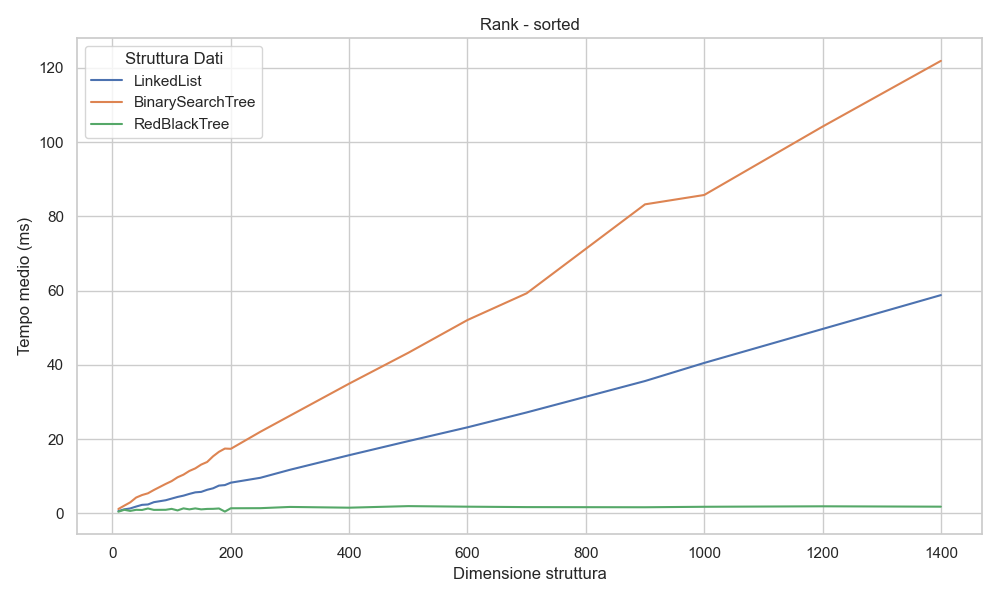
\includegraphics[width=0.8\linewidth]{plots/confronto/sorted_rank.png}
    \caption{Grafico del Rank con dati ordinati}
    \label{confronto-rank-sorted}
\end{figure}
\begin{table}[H]
\centering
\begin{tabular}{|c|c|c|c|}
\hline
\textbf{Size} & \textbf{Albero Binario} & \textbf{Lista Ordinata} & \textbf{Albero Rosso Nero} \\
\hline
10     & 1.174 & 0.616 & 0.44 \\
30     & 2.957 & 1.321  & 0.654 \\
180    & 16.57 & 7.473  & 1.311 \\
1400   & 121.9 & 58.78  & 1.796 \\
\hline
\end{tabular}
\caption{Tempi medi di esecuzione (ms) delle operazioni \texttt{Rank} con dati di input ordinati}
\label{tab:confronto-rank-sorted}
\end{table}

\subsubsection{dati ordinati al contrario}
Questo caso è stato preso in considerazione perché crea uno sbilanciamento dell'albero binario di ricerca, ma è il caso \textbf{migiore} della lista ordinata.
\begin{figure}[H]
    \centering
    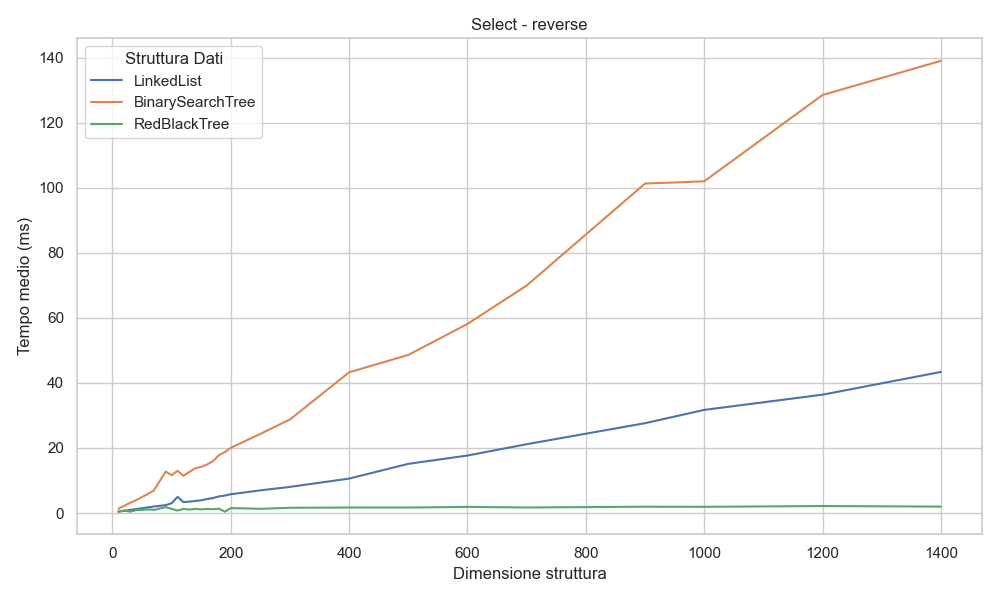
\includegraphics[width=0.8\linewidth]{plots/confronto/reverse_select.png}
    \caption{Grafico Select con dati ordinati al contrario}
    \label{confronto-select-reverse}
\end{figure}
\begin{table}[H]
\centering
\begin{tabular}{|c|c|c|c|}
\hline
\textbf{Size} & \textbf{Albero Binario} & \textbf{Lista Ordinata} & \textbf{Albero Rosso Nero} \\
\hline
10     & 1.309 & 0.423 & 0.411 \\
30     & 3.166 & 0.956  & 0.5 \\
180    & 17.79 & 5.111  & 1.341 \\
1400   & 139.1 & 43.38  & 1.969 \\
\hline
\end{tabular}
\caption{Tempi medi di esecuzione (ms) delle operazioni \texttt{Select} con dati di input ordinati al contrario}
\label{tab:confronto-select-reverse}
\end{table}
\begin{figure}[H]
    \centering
    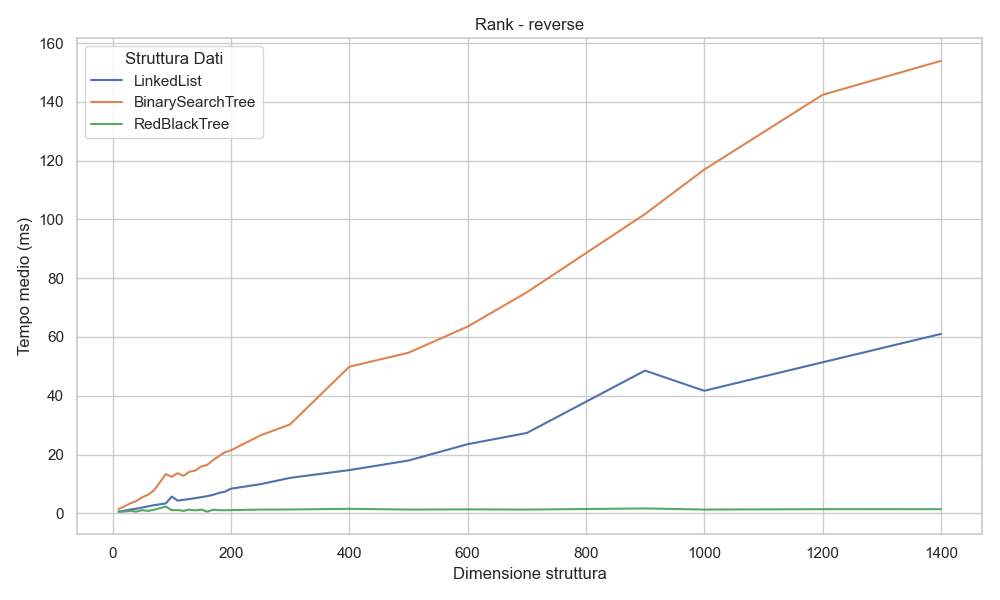
\includegraphics[width=0.8\linewidth]{plots/confronto/reverse_rank.png}
    \caption{Grafico Rank con dati ordinati al contrario}
    \label{confronto-rank-reverse}
\end{figure}
\begin{table}[H]
\centering
\begin{tabular}{|c|c|c|c|}
\hline
\textbf{Size} & \textbf{Albero Binario} & \textbf{Lista Ordinata} & \textbf{Albero Rosso Nero} \\
\hline
10     & 1.432 & 0.5313 & 0.5364 \\
30     & 3.382 & 1.265  & 0.797 \\
180    & 19.49 & 6.946  & 1.019 \\
1400   & 154 & 61.03  & 1.393 \\
\hline
\end{tabular}
\caption{Tempi medi di esecuzione (ms) delle operazioni \texttt{Rank} con dati di input ordinati al contrario}
\label{tab:confronto-rank-reverse}
\end{table}
\subsubsection{dati random con duplicati}
Questo caso è stato scelto per vedere se la presenza di duplicati influenzasse in modo positivo o negativo le funzioni di \textbf{Select} e \textbf{Rank} nelle diverse strutture dati. Qui mostreremo i risultati.
\begin{figure}[H]
    \centering
    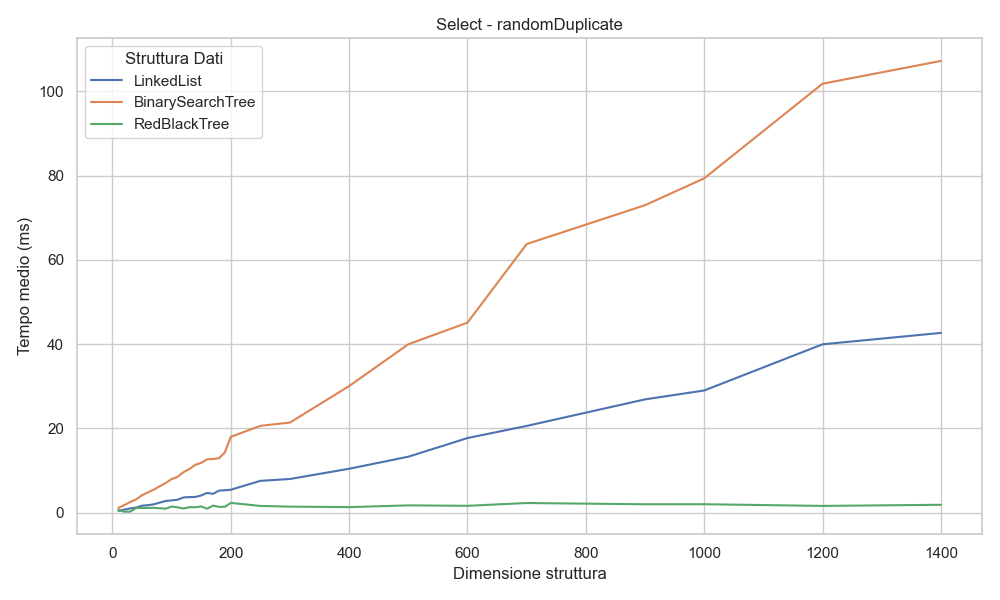
\includegraphics[width=0.8\linewidth]{plots/confronto/randomDuplicate_select.png}
    \caption{Grafico Select con dati random duplicati}
    \label{confronto-select-duplicated}
\end{figure}
\begin{table}[H]
\centering
\begin{tabular}{|c|c|c|c|}
\hline
\textbf{Size} & \textbf{Albero Binario} & \textbf{Lista Ordinata} & \textbf{Albero Rosso Nero} \\
\hline
10     & 1.118 & 0.442 & 0.6264 \\
30     & 2.523 & 1.004  & 0.89 \\
180    & 12.93 & 5.241  & 1.377 \\
1400   & 107.2 & 42.68  & 1.876 \\
\hline
\end{tabular}
\caption{Tempi medi di esecuzione (ms) delle operazioni \texttt{Select} con dati di input random duplicabili}
\label{tab:confronto-select-duplicated}
\end{table}
\begin{figure}
    \centering
    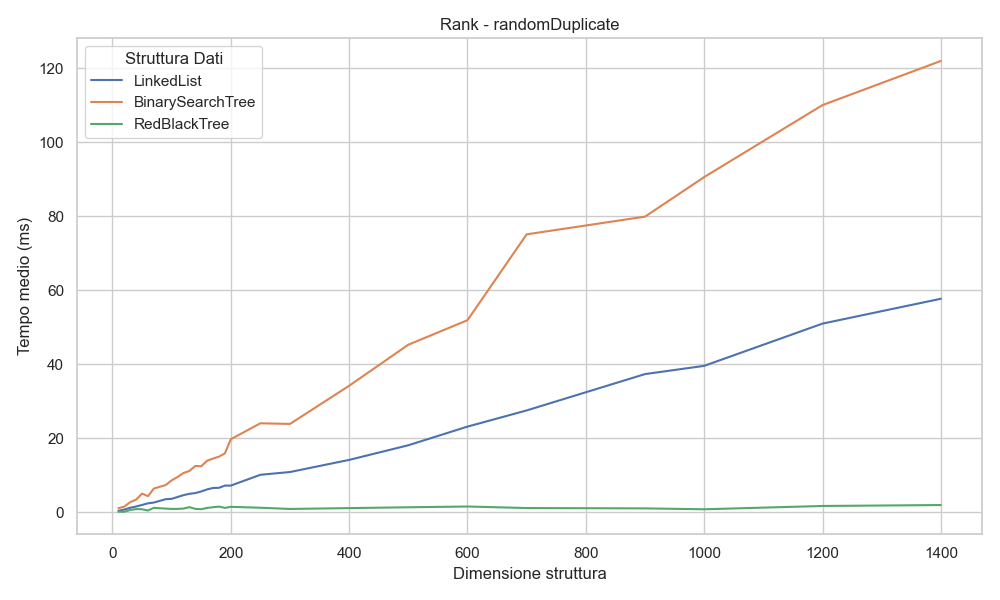
\includegraphics[width=0.8\linewidth]{plots/confronto/randomDuplicate_rank.png}
    \caption{Grafico Rank con dati random duplicati}
    \label{confronto-rank-duplicated}
\end{figure}
\begin{table}[H]
\centering
\begin{tabular}{|c|c|c|c|}
\hline
\textbf{Size} & \textbf{Albero Binario} & \textbf{Lista Ordinata} & \textbf{Albero Rosso Nero} \\
\hline
10     & 1.155 & 0.4584 & 0.223 \\
30     & 2.791 & 1.28  & 0.678 \\
180    & 15.09 & 6.67  & 1.595 \\
1400   & 122 & 57.73  & 2.013 \\
\hline
\end{tabular}
\caption{Tempi medi di esecuzione (ms) delle operazioni \texttt{Rank} con dati di input random duplicabili}
\label{tab:confronto-rank-duplicated}
\end{table}
\subsection{Approfondimenti risultati}
\label{approfondimenti}
All'interno della relazione per questione di rilevanza e di estetica non sono stati inseriti tutti i grafici ottenuti dai test, come ad esempio tutti i risultati delle tabelle o l'andamento di una singola struttura dati.\newline Per completezza inserisco dei link dove è possibile osservarli:
\begin{itemize}
    \item \href{https://github.com/Pennelli02/SelectRankValutation/tree/master/output/plots/table}{\textbf{Tabelle complete}}
    \item \href{https://github.com/Pennelli02/SelectRankValutation/tree/master/output/plots/BinarySearchTree}{\textbf{Albero Binario di Ricerca}}
    \item \href{https://github.com/Pennelli02/SelectRankValutation/tree/master/output/plots/LinkedList}{\textbf{Lista Ordinata}}
    \item \href{https://github.com/Pennelli02/SelectRankValutation/tree/master/output/plots/RedBlackTree}{\textbf{Albero Rosso Nero}}
\end{itemize}

\newpage
\subsection{Tesi e sintesi finale}
Osservando i risultati ottenuti dai test e proposti nella  \hyperref[risultati sperimentali]{sezione 4.2} possiamo dare le seguenti osservazioni:
\begin{itemize}
    \item i metodi di \textbf{select} e di \textbf{rank} nell'\textbf{albero binario di ricerca} e \textbf{lista ordinata} hanno complessità $O(n)$, mentre l'\textbf{albero rosso nero aumentato} dimostra una complessità $O(logn)$.
    \item la complessità dei metodi \textbf{select} e di \textbf{rank} non vengono influenzati se siamo nel caso migliore o peggiore di una struttura dati. Infatti, anche se l'\textbf{albero binario di ricerca} risulti sbilanciato esso ci mette sempre $O(n)$. Notiamo che la stessa cosa accade anche per la \textbf{lista ordinata}.
    L'ordine degli input e la loro distribuzione non influenza queste operazioni.
    \item L'\textbf{albero rosso-nero}, grazie al bilanciamento automatico e alla presenza dell'attributo \textbf{size}, risulta sistematicamente più efficiente rispetto alle altre strutture. Tuttavia, la sua elevata efficienza rende più difficile osservare chiaramente l'andamento asintotico, soprattutto in presenza di dataset di dimensioni ridotte.
\end{itemize}
\newpage
\begin{thebibliography}{9}
\bibitem{}
Thomas H. Cormen, Charles E. Leiserson, Ronald L. Rivest, Clifford Stein Introduzione agli algoritmi e strutture dati Terza edizione, McGraw Hill.

\end{thebibliography}   
\end{document}  